\documentclass[a4paper]{article}

\usepackage[utf8]{inputenc}
\usepackage[T1]{fontenc}
\usepackage{textcomp}
\usepackage[english]{babel}
\usepackage{amsmath, amssymb}
\usepackage[marginparwidth=1.75cm]{geometry}

% figure support
\usepackage{import}
\usepackage{xifthen}
\pdfminorversion=7
\usepackage{pdfpages}
\usepackage{transparent}
\usepackage{graphicx}
\newcommand{\incfig}[1]{%
		\def\svgwidth{\columnwidth}
		\import{./figures/}{#1.pdf_tex}
}

\pdfsuppresswarningpagegroup=1

\begin{document}
\title{E106 Cavities}
\maketitle 
	\section{Cavities Assignment}
	The cylindrical cavity has an inner diameter of 78.5mm and length of 20mm. From the lab script, we have the formula for resonant frequency as:
	\begin{equation}
			(d \nu)^2 = \left(\frac{cj^{(')}_{mn} }{\pi }\right)^2 + \left(\frac{c}{2}\right)^2 p^2 \left(\frac{d}{l}\right)^2 
			\label{eq:res_freq}
	\end{equation}
	
	Here $d = 2\cdot a$ is the diameter of the cavity and $j^{(')}_{mn}$ denotes the zero point Bessel function or its derivative. For TM modes it is zero point and for the TE modes, it is the derivative. 
	So we have, $\left(d/l\right)^2 = 15.405625$. Therefore, from the modemap, the ten lowest eigenmodes are:
	\begin{enumerate}
			\item $TM_{010} $ = 0.5e+17 \\ 
					$\nu = 2.848 GHz$ 
			\item $TM_{110} $ = 1.3e+17 \\ 
					$\nu = 4.593 GHz$ 
			\item $TM_{210} $ = 2.4e+17 \\ 
					$ \nu = 6.240 GHz$ 
			\item $TM_{020} $ = 2.8e+17 \\
					$\nu = 6.740 GHz$ 
			\item $TE_{111} $ = 3.6e+17 \\ 
					$\nu = 7.643 GHz$ 
			\item $TM_{310} $ = 3.7e+17 \\
					$\nu = 7.748 GHz$ 
			\item $TM_{011} $ = 3.9e+17 \\
					$\nu = 7.955 GHz$ 
			\item $TE_{211} $ = 4.3e+17 \\
					$\nu = 8.353 GHz$ 
			\item $TM_{120} $ = 4.5e+17 \\
					$\nu = 8.545 GHz$ 
			\item $TM_{111}/TE_{011}  $ = 4.7e+17 \\
					$\nu = 8.733 GHz$ 
	\end{enumerate}
	Now, we will calculate the resonant frequencies using Eq.\ref{eq:res_freq} and explicit values of the zeros of the Bessel function and its derivative below.
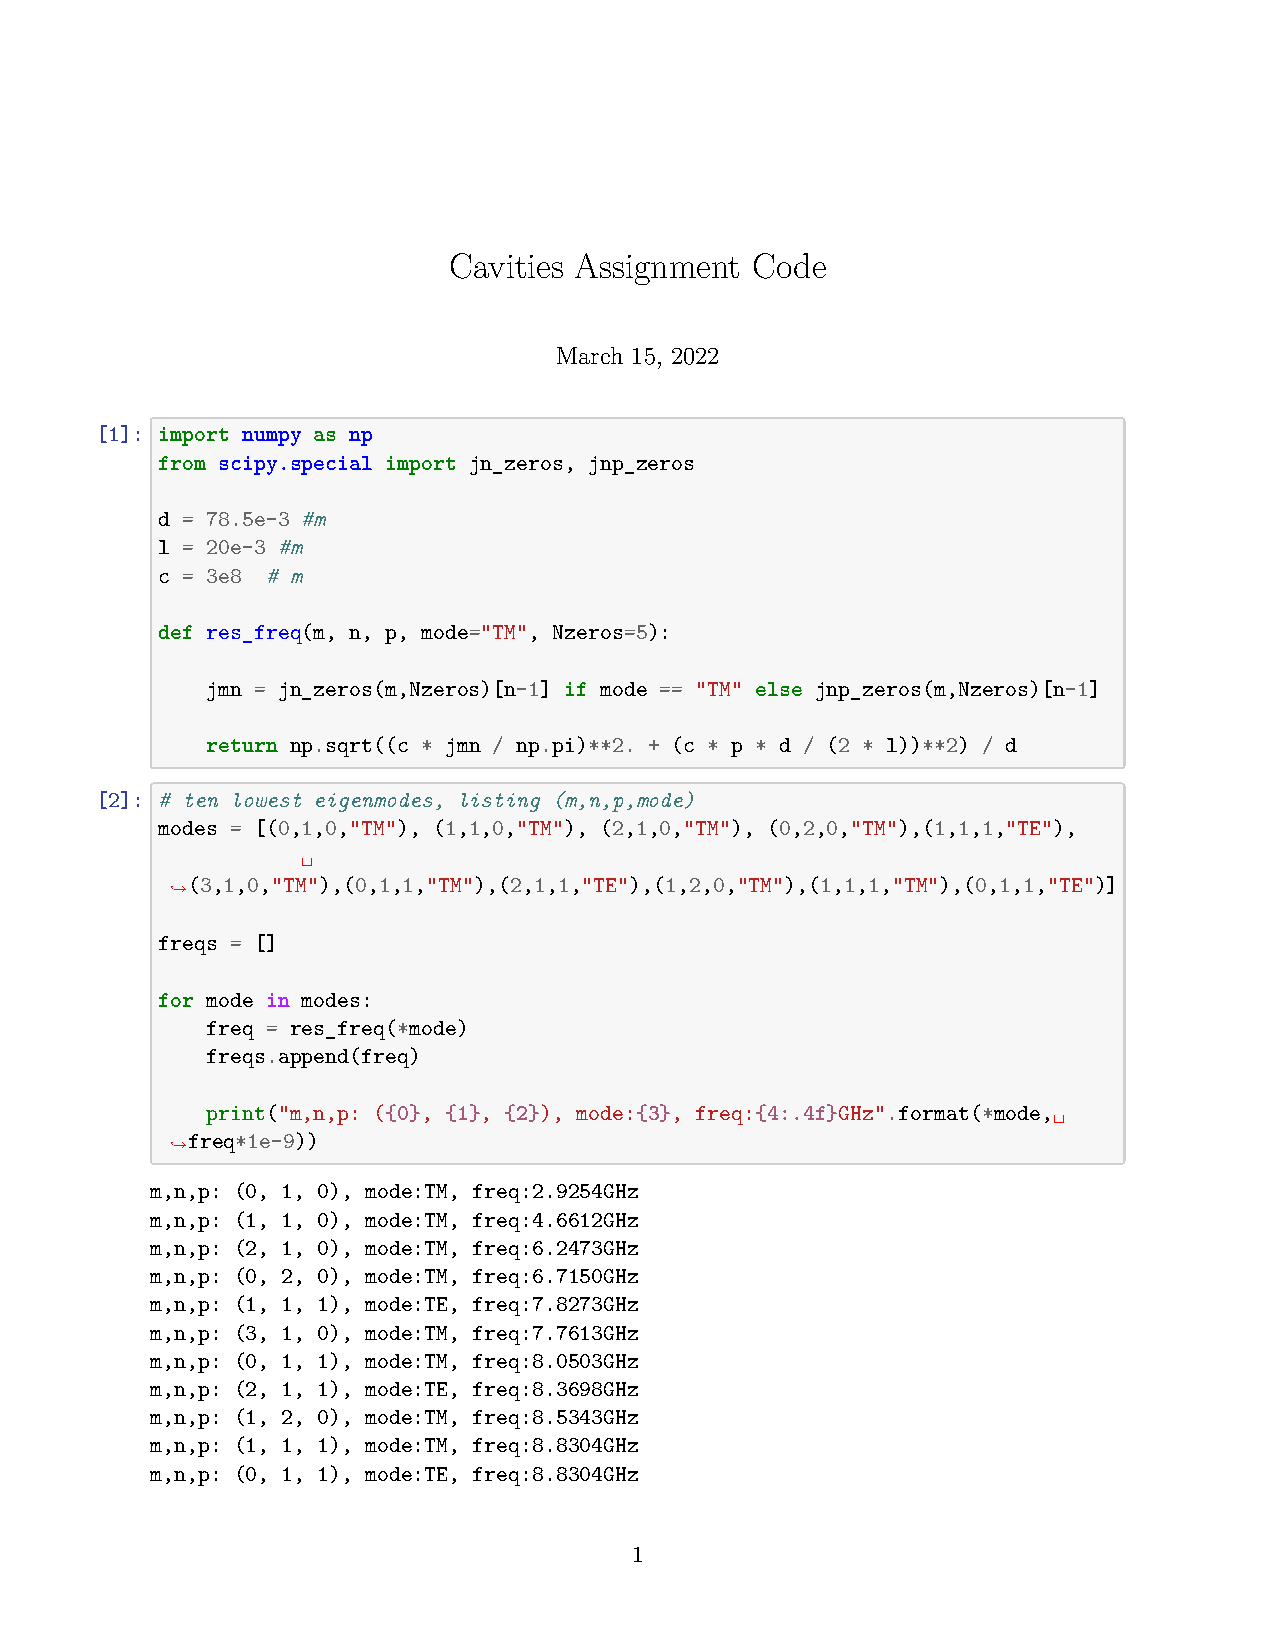
\includepdf[page=-]{Cavities Assignment Code}
\end{document}
